\documentclass[a4paper]{article}

\usepackage{enumitem, amsmath, gensymb, graphicx, caption, amssymb, geometry, fancyhdr, arydshln}
\usepackage[utf8]{inputenc}

\geometry{left=1in, right=1in, top=1in, bottom=1in}
\pagestyle{fancy}

\newcommand{\myName}{\textbf{Shantanu Ghodgaonkar}\\\textit{Univ ID}: N11344563\\\textit{Net ID}: sng8399\\\textit{Ph.No.}: +1 (929) 922-0614}
\newlist{qalist}{description}{1}
\setlist[qalist]{style=unboxed,leftmargin=0.5cm,labelwidth=2.5cm}


\title{Homework 1 Answers : ROB-GY 6003}
\author{\myName}
\date{\today}

%\fancyhf{} % Clear existing header/footer settings
\fancyhead{} % Clear existing header settings
\fancyhead[L]{\today}
%\fancyhead[C]{Center Header}
\fancyhead[R]{N11344563}
%\fancyfoot[R]{\thepage}


\begin{document}
	
	\begin{titlepage}
	    \centering
	    \vspace{2cm}
	    \Huge\textbf{Foundations of Robotics \\ ROB-GY 6003 \\ Homework 1 Answers}
	    \vspace{1cm}
	    \\ \Large \today
	    \vfill 
	    \Large \myName
	\end{titlepage}
	
	
	\begin{qalist}
		\item[Question: 2.1]
		\item[Answer:]
			It is given that a vector \textsuperscript{A}P is rotated about \( \hat{Z} \)\textsubscript{A} by $\theta$\degree, the roation matrix is given by - 

			\begin{equation}
			{R}_{Z} (\theta) = 
				\left[ \begin{matrix}
					\cos\theta & -\sin\theta & 0 \\
					\sin\theta & \cos\theta & 0 \\
					0 & 0 & 1
				\end{matrix} \right]
			\end{equation}
			
			The vector is subsequently rotated about \(\hat{X}\)\textsubscript{A} by $\phi$\degree, then the rotation matrix is given by - 
			
			\begin{equation}
			{R}_{Z X} (\theta,\phi) = 
				\left[ \begin{matrix}
					1 & 0 & 0 \\
					0 & \cos\phi & -\sin\phi\\
					0 & \sin\phi & \cos\phi\\
				\end{matrix} \right]
				\left[ \begin{matrix}
					\cos\theta & -\sin\theta & 0 \\
					\sin\theta & \cos\theta & 0 \\
					0 & 0 & 1
				\end{matrix} \right]
			\end{equation}
			
			\begin{equation}
			{R}_{Z X} (\theta,\phi) = 
				\left[ \begin{matrix}
					\cos\theta & -\sin\theta & 0 \\
					\cos\phi\sin\theta & \cos\phi\cos\theta & -\sin\theta\\
					\sin\phi\sin\theta & \sin\phi\cos\theta & \cos\phi\\
				\end{matrix} \right]
			\end{equation}
			
			
		\item[Question: 2.3] \setcounter{equation}{0}
		\item[Answer:]
			It is given that a frame \{B\} is rotated about \( \hat{Z} \)\textsubscript{B} by $\theta$\degree, the roation matrix is given by - 

			\begin{equation}
			{}^{A}_{B}{R}_{Z} (\theta) = 
				\left[ \begin{matrix}
					\cos\theta & -\sin\theta & 0 \\
					\sin\theta & \cos\theta & 0 \\
					0 & 0 & 1
				\end{matrix} \right]
			\end{equation}
			
			The frame {B} is subsequently rotated about \(\hat{X}\)\textsubscript{B} by $\phi$\degree, then the rotation matrix is given by - 
			
			\begin{equation}
			{}^{A}_{B}{R}_{Z X} (\theta,\phi) = 
				\left[ \begin{matrix}
					\cos\theta & -\sin\theta & 0 \\
					\sin\theta & \cos\theta & 0 \\
					0 & 0 & 1
				\end{matrix} \right]
				\left[ \begin{matrix}
					1 & 0 & 0 \\
					0 & \cos\phi & -\sin\phi\\
					0 & \sin\phi & \cos\phi\\
				\end{matrix} \right]
			\end{equation}
			\begin{equation}
			{}^{A}_{B}{R}_{Z X} (\theta,\phi) = 
				\left[ \begin{matrix}
					\cos\theta & -\sin\theta\cos\phi & \sin\theta\sin\phi \\
					\sin\theta & \cos\theta\cos\phi & -\cos\theta\sin\phi\\
					0 & \sin\phi & \cos\phi\\
				\end{matrix} \right]
			\end{equation}

		\item[Question: 2.12] \setcounter{equation}{0}
		\item[Answer:]
			Given : 
			
			A velocity vector 
			\begin{equation}
				{}^{B}{V} = 
				\left[ \begin{matrix}
					10.0 \\
					20.0 \\
					30.0
				\end{matrix} \right]
			\end{equation}		
			
			And a Transformation Operator, 
			\begin{equation}
				{}^{A}_{B}{T} = 
				\left[ \begin{matrix}
					0.866 & -0.500 &  0.000 & 11.0\\
					0.500 & 0.866 & 0.000 & -3.0\\
					0.000 & 0.000 & 1.000 & 9.0\\
					0 & 0 & 0 & 1
				\end{matrix} \right]
			\end{equation}
			
			As Velocity is a free vector, we have the relation (Eq\textsuperscript{n} 2.94), 
			\begin{equation}
				{}^{A}{V} = {}^{A}_{B}{R} {}^{B}{V}
			\end{equation}
			
			\begin{equation}
				{}^{A}{V} = \left[ \begin{matrix}
					0.866 & -0.500 &  0.000 \\
					0.500 & 0.866 & 0.000 \\
					0.000 & 0.000 & 1.000 
				\end{matrix} \right]
				\left[ \begin{matrix}
					10.0 \\
					20.0 \\
					30.0
				\end{matrix} \right]
			\end{equation}
			
			Finally,
			\begin{equation}
				{}^{A}{V} = 
				\left[ \begin{matrix}
					-1.34 \\
					22.32 \\
					30
				\end{matrix} \right]
			\end{equation}
			
		\item[Question: 2.14] \setcounter{equation}{0} 
		\item[Answer:]		
			Consider below Figure 1. \\
			\begin{minipage}{\linewidth}
				\centering
				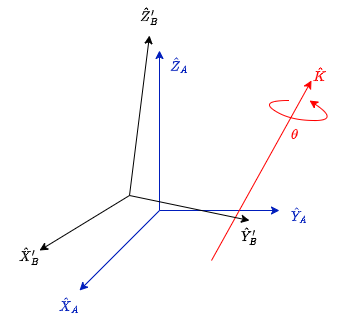
\includegraphics[width=0.45\textwidth]{2_14_Figure.drawio.png}
				\captionof{figure}{Frame $\{B\}$ rotated about a general axis $\hat{K}$ that does not pass through the origin of the original frame}
				\vspace{0.5cm}
			\end{minipage}
			
			In order for us to obtain a generalised formula, we shall use the one which we already know as Rodriques' Formula, 
			\begin{equation}
			{R}_{K}(\theta) = 
				\left[ \begin{matrix} 
					\textit{${k}_{x}{k}_{x}v\theta + c\theta$} & \textit{${k}_{x}{k}_{y}v\theta - {k}_{z}s\theta$} & \textit{${k}_{x}{k}_{z}v\theta + {k}_{y}s\theta$} \\
					\textit{${k}_{x}{k}_{y}v\theta + {k}_{z}s\theta$} & \textit{${k}_{y}{k}_{y}v\theta + c\theta$} & \textit{${k}_{y}{k}_{z}v\theta - {k}_{x}s\theta$} \\
					\textit{${k}_{x}{k}_{z}v\theta - {k}_{y}s\theta$} & \textit{${k}_{y}{k}_{z}v\theta + {k}_{x}s\theta$} & \textit{${k}_{z}{k}_{z}v\theta + c\theta$} \\
				\end{matrix} \right]
			\end{equation}
			
			But the above formula is for a general axis that passes through the origin of the initial coincidence.
			In order for us to use ${Eq}^{n} 1$ we will first have to translate the initial coincidence to a location that allows the general axis $\hat{K}$ to pass through its origin, then rotate the frame by the angle $\theta$ and then finally, undo the original translation, $i.e.$ bring it back to its original location.
			
			So, this transformation can be written as,
			\begin{equation}
				{}^{A}_{B}{T} = {D}_{Q}(q) {R}_{K}(\theta) {D}_{Q}(-q)
			\end{equation}
			
			Where, 
			\begin{equation}
				{D}_{Q}(q) = 
				\begin{bmatrix}
					1 & 0 & 0 & {q}_{x} \\
					0 & 1 & 0 & {q}_{y} \\
					0 & 0 & 1 & {q}_{z} \\
					0 & 0 & 0 & 1 \\
				\end{bmatrix}
			\end{equation}
			And, 
			\begin{equation}
				{D}_{Q}(-q) = 
				\left[ \begin{matrix}
					1 & 0 & 0 & -{q}_{x} \\
					0 & 1 & 0 & -{q}_{y} \\
					0 & 0 & 1 & -{q}_{z} \\
					0 & 0 & 0 & 1 \\
				\end{matrix}\right]
			\end{equation}
			
			Substituting ${Eq}^{n} 1$, ${Eq}^{n} 3$ and ${Eq}^{n} 4$ in ${Eq}^{n} 2$, we get, 
			\begin{equation}
				{}^{A}_{B}{T} = 
				\left[\begin{array}{ccc:c}
					{r}_{11} & {r}_{12} & {r}_{13} & {p}_{x}\\
					{r}_{21} & {r}_{22} & {r}_{23} & {p}_{y}\\
					{r}_{31} & {r}_{32} & {r}_{33} & {p}_{z}\\
					\hdashline
					0 & 0 & 0 & 1\\
				\end{array}\right]
			\end{equation}
			
			Where, ${r}_{ij}$ is given by ${Eq}^{n} 1$.
			\\And,
			\begin{equation}
				{p}_{x} = - {k}_{x} {q}_{x} - {k}_{y}{q}_{y} - {k}_{z}{q}_{z} + {q}_{x}
			\end{equation}
			\begin{equation}
				{p}_{y} = - {k}_{x} {q}_{x} - {k}_{y}{q}_{y} - {k}_{z}{q}_{z} + {q}_{y}
			\end{equation}
			\begin{equation}
				{p}_{z} = - {k}_{x} {q}_{x} - {k}_{y}{q}_{y} - {k}_{z}{q}_{z} + {q}_{z}
			\end{equation}
			
		\item[Question: 2.19] \setcounter{equation}{0} 
		\item[Answer:]
		Consider the below Figure 2.	\\				
			\begin{minipage}{\linewidth}
				\centering
				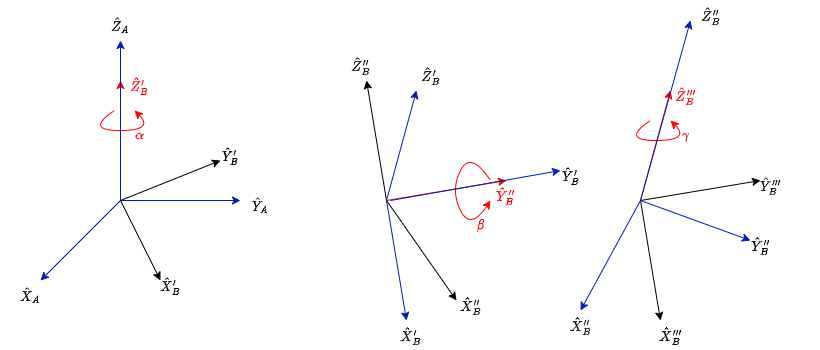
\includegraphics[width=1\textwidth]{zyzEulerAngles.drawio.png}
				\captionof{figure}{Z-Y-Z Euler Angles}
			\end{minipage}
			Start with the frame coincident with a known frame $A$. Rotate $B$ first about $\hat{Z}_{B}$ by an angle $\alpha$, then about $\hat{Y}_{B}$ by an angle $\beta$, and, finally, about $\hat{Z}_{B}$ by an angle $\gamma$ . (See above Figure 1) \\
			
			A rotation matrix parameterised by Z-Y-Z Euler angles is indicated by the notation ${}^{A}_{B}{R}_{Z'Y'Z'}(\alpha, \beta, \gamma)$
			
			With reference to \textit{Figure 1}, we can ues the intermediate frames $\{B'\}$, $\{B''\}$ and $\{B'''\}$ in order to give an expression for the rotation matrix ${}^{A}_{B}{R}_{Z'Y'Z'}(\alpha, \beta, \gamma)$.
			
			The first rotation, from $\{A\}$ to $\{B'\}$ is given by,
			\begin{equation}
				{}^{A}_{B'}{R} = {R}_{Z}(\alpha)
			\end{equation}
			The second rotation, now expressed in fixed coordinates is, 
			\begin{equation}
				{}^{B'}_{B''}{R} = {R}_{Z}(\alpha){R}_{Y}(\beta){R}^{-1}_{Z}(\alpha)
			\end{equation}
			And the third rotation is given by,
			\begin{equation}
				{}^{B''}_{B'''}{R} =({R}_{Z}(\alpha){R}_{Y}(\beta){R}^{-1}_{Z}(\alpha)) {R}_{Z}(\gamma) {({R}_{Z}(\alpha){R}_{Y}(\beta){R}^{-1}_{Z}(\alpha))}^{-1}
			\end{equation}
			The result, 
			\begin{equation}
				{}^{A}_{B}{R} =  {}^{B''}_{B}{R}\;{}^{B'}_{B''}{R}\;{}^{A}_{B'}{R}
			\end{equation}
			Upon substituting ${Eq}^{n}1$, ${Eq}^{n}2$ and ${Eq}^{n}3$ in ${Eq}^{n}4$, we get, 
			\begin{equation}
				\Rightarrow {}^{A}_{B}{R}_{Z'Y'Z'}(\alpha, \beta, \gamma) = {R}_{Z}(\alpha){R}_{Y}(\beta){R}_{Z}(\gamma)
			\end{equation}
			\begin{equation}
				= \left[ \begin{matrix}
					\cos\alpha && -\sin\alpha && 0 \\
					\sin\alpha && \cos\alpha && 0 \\
					0 && 0 && 1
				\end{matrix}\right]
				\left[ \begin{matrix}
					\cos\beta && 0 && \sin\beta \\
					0 && 1 && 0 \\
					-\sin\beta && 0 && \cos\beta
				\end{matrix}\right]
				\left[ \begin{matrix}
					\cos\gamma && -\sin\gamma && 0 \\
					\sin\gamma && \cos\gamma && 0 \\
					0 && 0 && 1
				\end{matrix}\right]
			\end{equation}			
			\begin{equation}
				\therefore {}^{A}_{B}{R}_{Z'Y'Z'}(\alpha, \beta, \gamma) =
				\left[\begin{matrix}
					\cos\alpha\cos\beta\cos\gamma -\sin\alpha\sin\gamma & -\cos\alpha\cos\beta\sin\gamma-\sin\alpha\cos\gamma & \cos\alpha\sin\beta \\
					\sin\alpha\cos\beta\cos\gamma+\cos\alpha\sin\gamma & -\sin\alpha\cos\beta\sin\gamma+\cos\alpha\cos\gamma & \sin\alpha\sin\beta \\
					-\sin\beta\cos\gamma & \sin\beta\sin\gamma & \cos\beta
				\end{matrix}\right]
			\end{equation}
			
		
		\item[Question: 2.20] \setcounter{equation}{0}
		\item[Answer:] 
		It is given that a vector \textit{Q} rotates about a vect \( \hat{K} \) by $\theta$\degree to form a new vector \textit{Q'}, given by the equation,
		\begin{equation}
			\textit{Q'} = \textit{${R}_{K}(\theta)$Q}
		\end{equation}
		Let us start with Equation (2.80), 
		\begin{equation}
			{R}_{K}(\theta) = 
				\left[ \begin{matrix} 
					\textit{${k}_{x}{k}_{x}v\theta + c\theta$} & \textit{${k}_{x}{k}_{y}v\theta - {k}_{z}s\theta$} & \textit{${k}_{x}{k}_{z}v\theta + {k}_{y}s\theta$} \\
					\textit{${k}_{x}{k}_{y}v\theta + {k}_{z}s\theta$} & \textit{${k}_{y}{k}_{y}v\theta + c\theta$} & \textit{${k}_{y}{k}_{z}v\theta - {k}_{x}s\theta$} \\
					\textit{${k}_{x}{k}_{z}v\theta - {k}_{y}s\theta$} & \textit{${k}_{y}{k}_{z}v\theta + {k}_{x}s\theta$} & \textit{${k}_{z}{k}_{z}v\theta + c\theta$} \\
				\end{matrix} \right]
		\end{equation}
		
		\begin{equation} = 
				\left[ \begin{matrix} 
					\textit{${k}_{x}{k}_{x}v\theta$} & \textit{${k}_{x}{k}_{y}v\theta$} & \textit{${k}_{x}{k}_{z}v\theta$} \\
					\textit{${k}_{x}{k}_{y}v\theta$} & \textit{${k}_{y}{k}_{y}v\theta$} & \textit{${k}_{y}{k}_{z}v\theta$} \\
					\textit{${k}_{x}{k}_{z}v\theta$} & \textit{${k}_{y}{k}_{z}v\theta$} & \textit{${k}_{z}{k}_{z}v\theta$} \\
				\end{matrix} \right]
				+
				\left[ \begin{matrix} 
					\textit{$c\theta$} & \textit{$- {k}_{z}s\theta$} & \textit{${k}_{y}s\theta$} \\
					\textit{${k}_{z}s\theta$} & \textit{$c\theta$} & \textit{$- {k}_{x}s\theta$} \\
					\textit{$- {k}_{y}s\theta$} & \textit{${k}_{x}s\theta$} & \textit{$c\theta$} \\
				\end{matrix} \right]
		\end{equation}
		
		\begin{equation} = 
				v\theta\left[ \begin{matrix} 
					\textit{${k}_{x}{k}_{x}$} & \textit{${k}_{x}{k}_{y}$} & \textit{${k}_{x}{k}_{z}$} \\
					\textit{${k}_{x}{k}_{y}$} & \textit{${k}_{y}{k}_{y}$} & \textit{${k}_{y}{k}_{z}$} \\
					\textit{${k}_{x}{k}_{z}$} & \textit{${k}_{y}{k}_{z}$} & \textit{${k}_{z}{k}_{z}$} 
				\end{matrix} \right]
				+
				\left[ \begin{matrix} 
					\textit{$c\theta$} & \textit{$- {k}_{z}s\theta$} & \textit{${k}_{y}s\theta$} \\
					\textit{${k}_{z}s\theta$} & \textit{$c\theta$} & \textit{$- {k}_{x}s\theta$} \\
					\textit{$- {k}_{y}s\theta$} & \textit{${k}_{x}s\theta$} & \textit{$c\theta$} \\
				\end{matrix} \right]
		\end{equation}
		
		\begin{equation} = 
				v\theta\left[ \begin{matrix} 
					\textit{${k}_{x}{k}_{x}$} & \textit{${k}_{x}{k}_{y}$} & \textit{${k}_{x}{k}_{z}$} \\
					\textit{${k}_{x}{k}_{y}$} & \textit{${k}_{y}{k}_{y}$} & \textit{${k}_{y}{k}_{z}$} \\
					\textit{${k}_{x}{k}_{z}$} & \textit{${k}_{y}{k}_{z}$} & \textit{${k}_{z}{k}_{z}$} 
				\end{matrix} \right]
				+
				\left[ \begin{matrix} 
					\textit{0} & \textit{$- {k}_{z}s\theta$} & \textit{${k}_{y}s\theta$} \\
					\textit{${k}_{z}s\theta$} & \textit{0} & \textit{$- {k}_{x}s\theta$} \\
					\textit{$- {k}_{y}s\theta$} & \textit{${k}_{x}s\theta$} & \textit{0} \\
				\end{matrix} \right]
				+
				\left[ \begin{matrix} 
					\textit{$c\theta$} & \textit{0} & \textit{0} \\
					\textit{0} & \textit{$c\theta$} & \textit{0} \\
					\textit{0} & \textit{0} & \textit{$c\theta$} \\
				\end{matrix} \right]
		\end{equation}
		
		
		\begin{equation} = 
				v\theta\left[ \begin{matrix} 
					\textit{${k}_{x}{k}_{x}$} & \textit{${k}_{x}{k}_{y}$} & \textit{${k}_{x}{k}_{z}$} \\
					\textit{${k}_{x}{k}_{y}$} & \textit{${k}_{y}{k}_{y}$} & \textit{${k}_{y}{k}_{z}$} \\
					\textit{${k}_{x}{k}_{z}$} & \textit{${k}_{y}{k}_{z}$} & \textit{${k}_{z}{k}_{z}$} 
				\end{matrix} \right]
				+
				s\theta\left[ \begin{matrix} 
					\textit{0} & \textit{$- {k}_{z}$} & \textit{${k}_{y}$} \\
					\textit{${k}_{z}$} & \textit{0} & \textit{$- {k}_{x}$} \\
					\textit{$- {k}_{y}$} & \textit{${k}_{x}$} & \textit{0}
				\end{matrix} \right]
				+
				c\theta\left[ \begin{matrix} 
					\textit{1} & \textit{0} & \textit{0} \\
					\textit{0} & \textit{1} & \textit{0} \\
					\textit{0} & \textit{0} & \textit{1} \\
				\end{matrix} \right]
		\end{equation}
		
		Substituting above equation in equation (1), 
		
		\begin{equation} \textit{Q'}= \left(
				v\theta\left[ \begin{matrix} 
					\textit{${k}_{x}{k}_{x}$} & \textit{${k}_{x}{k}_{y}$} & \textit{${k}_{x}{k}_{z}$} \\
					\textit{${k}_{x}{k}_{y}$} & \textit{${k}_{y}{k}_{y}$} & \textit{${k}_{y}{k}_{z}$} \\
					\textit{${k}_{x}{k}_{z}$} & \textit{${k}_{y}{k}_{z}$} & \textit{${k}_{z}{k}_{z}$} 
				\end{matrix} \right]
				+
				s\theta\left[ \begin{matrix} 
					\textit{0} & \textit{$- {k}_{z}$} & \textit{${k}_{y}$} \\
					\textit{${k}_{z}$} & \textit{0} & \textit{$- {k}_{x}$} \\
					\textit{$- {k}_{y}$} & \textit{${k}_{x}$} & \textit{0}
				\end{matrix} \right]
				+
				c\theta\left[ \begin{matrix} 
					\textit{1} & \textit{0} & \textit{0} \\
					\textit{0} & \textit{1} & \textit{0} \\
					\textit{0} & \textit{0} & \textit{1} \\
				\end{matrix} \right] \right) \textit{Q}
		\end{equation}
		
		\begin{equation} = 
				Qv\theta\left[ \begin{matrix} 
					\textit{${k}_{x}{k}_{x}$} & \textit{${k}_{x}{k}_{y}$} & \textit{${k}_{x}{k}_{z}$} \\
					\textit{${k}_{x}{k}_{y}$} & \textit{${k}_{y}{k}_{y}$} & \textit{${k}_{y}{k}_{z}$} \\
					\textit{${k}_{x}{k}_{z}$} & \textit{${k}_{y}{k}_{z}$} & \textit{${k}_{z}{k}_{z}$} 
				\end{matrix} \right]
				+
				Qs\theta\left[ \begin{matrix} 
					\textit{0} & \textit{$- {k}_{z}$} & \textit{${k}_{y}$} \\
					\textit{${k}_{z}$} & \textit{0} & \textit{$- {k}_{x}$} \\
					\textit{$- {k}_{y}$} & \textit{${k}_{x}$} & \textit{0}
				\end{matrix} \right]
				+
				Qc\theta\left[ \begin{matrix} 
					\textit{1} & \textit{0} & \textit{0} \\
					\textit{0} & \textit{1} & \textit{0} \\
					\textit{0} & \textit{0} & \textit{1} \\
				\end{matrix} \right]  
		\end{equation}
		
		Converting the matrices to their vector notation and substituting for \\$v\theta = 1 - \cos\theta$, we get,
		
		\begin{equation} = 
				(1-\cos\theta)\hat{K} \times \hat{K} \times Q
				+
				\sin\theta (\hat{K} \times Q)
				+
				Q\cos\theta
		\end{equation}
		
		Rearranging equation (9)
		\begin{equation}
			Q' = Q\cos\theta + \sin\theta(\hat{K} \times Q) + (1 - \cos\theta)(\hat{K} \cdot Q) \hat{K}
		\end{equation}
		
		Equation (9) represents Rodriques's Formula, with equation (2) being the matrix representation of the same.\\
		\textbf{QED} 
		
		\newpage
		\item[Question: 2.21] \setcounter{equation}{0} 
		\item[Answer:]
			Given, 
			\begin{equation}
			{R}_{K}(\theta) = 
				\left[ \begin{matrix} 
					\textit{${k}_{x}{k}_{x}v\theta + c\theta$} & \textit{${k}_{x}{k}_{y}v\theta - {k}_{z}s\theta$} & \textit{${k}_{x}{k}_{z}v\theta + {k}_{y}s\theta$} \\
					\textit{${k}_{x}{k}_{y}v\theta + {k}_{z}s\theta$} & \textit{${k}_{y}{k}_{y}v\theta + c\theta$} & \textit{${k}_{y}{k}_{z}v\theta - {k}_{x}s\theta$} \\
					\textit{${k}_{x}{k}_{z}v\theta - {k}_{y}s\theta$} & \textit{${k}_{y}{k}_{z}v\theta + {k}_{x}s\theta$} & \textit{${k}_{z}{k}_{z}v\theta + c\theta$} \\
				\end{matrix} \right]
			\end{equation}
			And the applying the approximations: 
				$\sin\theta = \theta$,
				$\cos\theta = 1$,
				$\theta^{2} = 0$,\\
				$v\theta = 1 - \cos\theta = 1 - 1 = 0$
			to the Equation (1), we get,
			
			\begin{equation}
				{R}_{K}(\theta) = 
				\left[ \begin{matrix} 
					\textit{${k}_{x}{k}_{x}(0) + 1$} & \textit{${k}_{x}{k}_{y}(0) - {k}_{z}\theta$} & \textit{${k}_{x}{k}_{z}(0) + {k}_{y}\theta$} \\
					\textit{${k}_{x}{k}_{y}(0) + {k}_{z}\theta$} & \textit{${k}_{y}{k}_{y}(0) + 1$} & \textit{${k}_{y}{k}_{z}(0) - {k}_{x}\theta$} \\
					\textit{${k}_{x}{k}_{z}(0) - {k}_{y}\theta$} & \textit{${k}_{y}{k}_{z}(0) + {k}_{x}\theta$} & \textit{${k}_{z}{k}_{z}(0) + 1$} \\
				\end{matrix} \right]
			\end{equation}
			
			\begin{equation}
				{R}_{K}(\theta) = 
				\left[ \begin{matrix} 
					\textit{$1$} & \textit{$ - {k}_{z}\theta$} & \textit{${k}_{y}\theta$} \\
					\textit{${k}_{z}\theta$} & \textit{$1$} & \textit{$-{k}_{x}\theta$} \\
					\textit{$- {k}_{y}\theta$} & \textit{${k}_{x}\theta$} & \textit{$1$} \\
				\end{matrix} \right]
			\end{equation}
			

		\item[Question: 2.22] \setcounter{equation}{0}
		\item[Answer:]
			Consider the answer of the previous question, 
			
			\begin{equation}
				{R}_{K}(\theta) = 
				\left[ \begin{matrix} 
					\textit{$1$} & \textit{$ - {k}_{z}\theta$} & \textit{${k}_{y}\theta$} \\
					\textit{${k}_{z}\theta$} & \textit{$1$} & \textit{${k}_{x}\theta$} \\
					\textit{$- {k}_{y}\theta$} & \textit{${k}_{x}\theta$} & \textit{$1$} \\
				\end{matrix} \right]
			\end{equation}
			
			Now, consider two rotations R\textsubscript{1} = ${R}_{A}(\alpha)$ and R\textsubscript{2} = ${R}_{B}(\beta)$.
			\\Such that, $\alpha << 1$ and $\beta <<1$ and $\alpha\beta \approx 0$
			
			If we form the product of the two rotations, \textit{i.e}, perform ${R}_{1}$ and then ${R}_{2}$
			\begin{equation}
				{R}_{1}{R}_{2} = 
				\left[ \begin{matrix} 
					\textit{$1$} & \textit{$ - {a}_{z}\alpha$} & \textit{${a}_{y}\alpha$} \\
					\textit{${a}_{z}\alpha$} & \textit{$1$} & \textit{${a}_{x}\alpha$} \\
					\textit{$- {a}_{y}\alpha$} & \textit{${a}_{x}\alpha$} & \textit{$1$}
				\end{matrix} \right]
				\left[ \begin{matrix} 
					\textit{$1$} & \textit{$ - {b}_{z}\beta$} & \textit{${b}_{y}\beta$} \\
					\textit{${b}_{z}\beta$} & \textit{$1$} & \textit{${b}_{x}\beta$} \\
					\textit{$- {b}_{y}\beta$} & \textit{${b}_{x}\beta$} & \textit{$1$}
				\end{matrix} \right]
			\end{equation}
			
			\begin{equation}
				= 
				\left[ \begin{matrix}
				1 && \textit{$ - {a}_{z}\alpha  - {b}_{z}\beta$} && \textit{${a}_{y}\alpha  + {b}_{y}\beta$} \\
				\textit{${a}_{z}\alpha  + {b}_{z}\beta$} && 1 && \textit{$ - {a}_{x}\alpha  - {b}_{x}\beta$} \\
				\textit{$ - {a}_{y}\alpha  - {b}_{y}\beta$} && \textit{${a}_{x}\alpha + {b}_{x}\beta$} && 1
				\end{matrix}\right]
			\end{equation}
			
			Now let's perform the two roations in the opposite order, 
			\begin{equation}
				{R}_{2}{R}_{1} = 
				\left[ \begin{matrix} 
					\textit{$1$} & \textit{$ - {b}_{z}\beta$} & \textit{${b}_{y}\beta$} \\
					\textit{${b}_{z}\beta$} & \textit{$1$} & \textit{${b}_{x}\beta$} \\
					\textit{$- {b}_{y}\beta$} & \textit{${b}_{x}\beta$} & \textit{$1$}
				\end{matrix} \right]
				\left[ \begin{matrix} 
					\textit{$1$} & \textit{$ - {a}_{z}\alpha$} & \textit{${a}_{y}\alpha$} \\
					\textit{${a}_{z}\alpha$} & \textit{$1$} & \textit{${a}_{x}\alpha$} \\
					\textit{$- {a}_{y}\alpha$} & \textit{${a}_{x}\alpha$} & \textit{$1$}
				\end{matrix} \right]
			\end{equation}
			
			\begin{equation}
				= 
				\left[ \begin{matrix}
				1 && \textit{$ - {a}_{z}\alpha  - {b}_{z}\beta$} && \textit{${a}_{y}\alpha  + {b}_{y}\beta$} \\
				\textit{${a}_{z}\alpha  + {b}_{z}\beta$} && 1 && \textit{$ - {a}_{x}\alpha  - {b}_{x}\beta$} \\
				\textit{$ - {a}_{y}\alpha  - {b}_{y}\beta$} && \textit{${a}_{x}\alpha + {b}_{x}\beta$} && 1
				\end{matrix}\right]
			\end{equation}
			
			Thus, upon comparing equations (3) and (5) we see that, 
						\begin{equation}
				{R}_{1}{R}_{2} = {R}_{2}{R}_{1} \end{equation}
				
			Therefore, we can say that two infinitesimal rotations commute.\\
			\textbf{QED} 
			\newpage

		\item[Question: 2.27] \setcounter{equation}{0}
		\item[Answer:]
			We are given the following Figure 2.25 - \\
			\begin{minipage}{\linewidth}
					\centering
					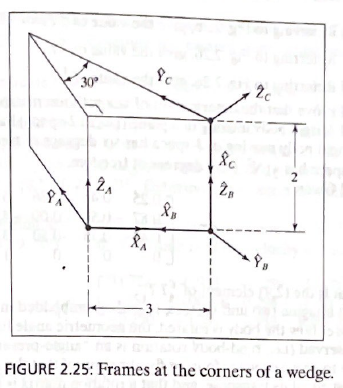
\includegraphics[width=0.5\textwidth]{fig225.png}
			\end{minipage}
			\\
			Referring to the given figure, we can see that the distance between frame \{A\} and \{B\} is that of 3\\
			And that with respect to frame \{A\}, frame \{B\} has rotated about \(\hat{Z}\) by 180\degree \\ \\
			And using Homogenous Transform Equation, \\ \\
			\begin{minipage}{\linewidth}
					\centering
					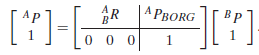
\includegraphics[width=0.5\textwidth]{HT.png}
			\end{minipage}
			\\ \\
			We get the matrix
			\begin{equation}
				{}^{A}_{B}{T} = 
				\left[ \begin{matrix}
					\cos(180) & -\sin(180) & 0 & 3 \\
					\sin(180) & \cos(180) & 0 & 0 \\
					0 & 0 & 1 & 0 \\
					0 & 0 & 0 & 1
				\end{matrix} \right]
			\end{equation}
			\begin{equation}
				{}^{A}_{B}{T} = 
				\left[ \begin{matrix}
					-1 & 0 & 0 & 3 \\
					0 & -1 & 0 & 0 \\
					0 & 0 & 1 & 0 \\
					0 & 0 & 0 & 1
				\end{matrix} \right]
			\end{equation}
		\item[Question: 2.37] \setcounter{equation}{0}
		\item[Answer:]		
			We know that a homogenous transform given by, \\
			\begin{equation}
			{}^{A}_{B}{T} = \raisebox{-0.5\height}{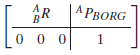
\includegraphics[width=0.3\textwidth]{HT_eqn.png}}
			\end{equation}
			And that the inverse of the transformation is given by, \\
			\begin{minipage}{\linewidth}
					\centering
				\begin{equation}	\raisebox{-0.5\height}{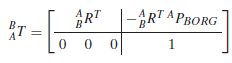
\includegraphics[width=0.5\textwidth]{HT_eqn_inv.png}} \end{equation}
			\end{minipage}
			Applying Equation (2) on the given homogenous transform, 
			\begin{equation}
				{}^{A}_{B}{T} = 
				\left[ \begin{matrix}
					0.25 & 0.43 & 0.86 & 5.0 \\
					0.87 & -0.5 & 0.00 & -4.0 \\
					0.43 & 0.75 & -0.5 & 3.0\\
					0 & 0 & 0 & 1
				\end{matrix} \right]
			\end{equation}
			We get, 
			\begin{equation}
				{}^{B}_{A}{T} = 
				\left[ \begin{matrix}
					0.25 & 0.87 & 0.43 & 0.94 \\
					0.43 & -0.5 & 0.75 & -6.4 \\
					0.86 & 0.00 & -0.5 & -2.8\\
					0 & 0 & 0 & 1
				\end{matrix} \right]
			\end{equation}
			Therefore, the (2,4) element of ${}^{B}_{A}{T}$ = -6.4
			
			
		\item[Question: 2.38] \setcounter{equation}{0}
		\item[Answer:]						
			We are given two vectors ${v}_{1}$ and ${v}_{2}$ embedded in a rigid body such that the geometric angle between the two is constant, immaterial of the number and order of rotations that the body undergoes. \\
			So, we can deduce that the scalar product of the two vectors remains constant.
			\begin{equation}{v}_{1} \cdot {v}_{2} = \cos\theta\end{equation}  Where $\theta$ is the angle between ${v}_{1} \& {v}_{2}$.\\
			${Eq}^{n} (1)$ can be rewritten in matrix form as,
			\begin{equation}{v}^{T}_{1}{v}_{2} = \cos\theta\end{equation} 
			Now, let us rotate the given rigid body. ${Eq}^{n} (2)$ can now be written as,
			\begin{equation}{(R{v}_{1})}^{T}({Rv}_{2}) = \cos\theta\end{equation} 
			But we know that $\cos\theta = {v}^{T}_{1}{v}_{2}$ (From ${Eq}^{n} (1)$),
			\begin{equation}{R}^{T}{v}^{T}_{1}R{v}_{2} = {v}^{T}_{1}{v}_{2}\end{equation} 
			Cancelling out ${v}^{T}_{1}{v}_{2}$ from both sides, we get,
			\begin{equation}{R}^{T}R = I\end{equation} 
			Where, $I$ represents the Identity Matrix. \\But we also know that by definition, the inverse of a matrix can be expressed as, 
			\begin{equation}{R}^{-1}R = I\end{equation}
			By comparing ${Eq}^{n} (5)$ and ${Eq}^{n} (6)$, we can see that,
			\begin{equation}{R}^{T} = {R}^{-1}\end{equation} 
			\textbf{QED.}
	\end{qalist}
\end{document}








